\documentclass[12pt]{book}
\usepackage[hmargin=0.6in,vmargin=1in]{geometry}
\usepackage{amsmath}
\usepackage{amsthm}
\usepackage[rightcaption]{sidecap}
\usepackage{graphicx}
\usepackage{placeins}
\usepackage{enumerate}
\usepackage{amssymb}
\usepackage{wrapfig}
\usepackage[dvipsnames]{xcolor}
\usepackage{tikz,lipsum,lmodern}
\usepackage[most]{tcolorbox}
\usepackage{hyperref}
\hypersetup{
    colorlinks=true,
    linkcolor=blue,
    filecolor=magenta,
    urlcolor=cyan,
}
\usepackage{setspace}
\title{Using fancyhdr for Custom Page Header and Footers in a Two-sided Document}

\usepackage{etoolbox}
\makeatletter
% no new page for \chapter
\patchcmd{\chapter}{\if@openright\cleardoublepage\else\clearpage\fi}{}{}{}
% don't change the pagestyle
\patchcmd{\chapter}{\thispagestyle{plain}}{}{}{%
    % example for a warning, 'Package' in text necessary to make TexStudio show it.
    \GenericWarning{(preamble)\@spaces\@spaces\@spaces\@spaces}{Package preamble Warning: patching \string\chapter\space did not work.}}

% allow floats on top of the page with a new chapter
\patchcmd{\chapter}{\global\@topnum\z@}{}{}{}
% if not commented out, first paragraph will be indented
\patchcmd{\chapter}{\@afterindentfalse}{}{}{}
%\makeatother

\usepackage{titlesec}
\titleformat{\chapter}{\normalfont\bfseries\Large}{\thechapter.\quad}{0pt}{}
\titlespacing{\chapter}{0pt}{2pt}{4pt}% left space, top space, bottom space



\usepackage{fancyhdr}
% Clear off all default fancyhdr headers and footers
\fancyhf{}
\pagestyle{fancy}

\addtolength{\headheight}{\baselineskip}

\fancyhead[L]{\leftmark}
\renewcommand{\chaptermark}[1]{\markboth{\MakeUppercase{#1}}{}}
%\fancyhead[L]{\textbf{\sectiontitle}}
\fancyhead[R]{\sffamily\itshape Lecture Notes on Biophysics}
% Custom text at the left edge of odd pages, and right edge of odd pages.
%\fancyhead[LO,RE]{\sffamily\itshape Fun with fancyhdr}

% Repeat for \fancyfoot if needed, e.g.
% Some decorative symbol at the centre of both odd and even pages
\fancyfoot[L]{\sffamily\itshape Linn Abraham , MGM College of Nursing}
\fancyfoot[C]{\thepage}
\fancyfoot[R]{ September 2020}
% Set this length to 0pt if you don't want any lines!
\renewcommand{\headrulewidth}{2pt}
%\pagenumbering{roman}
% Apply the fancy header style
\onehalfspacing

\usepackage{lipsum}
\begin{document}
\setcounter{secnumdepth}{0}

\title{Nuclear Physics}
\maketitle
\tableofcontents
\newpage

\setcounter{page}{1}
\graphicspath{ {../} }
\chapter{Atoms}
\section{Planetary model of atom}
\begin{itemize}
	\item Rutherford proposed the planetary model of the atom.
	\item The planetary model of the atom pictures low-mass electrons orbiting a large-mass nucleus.
	\item The sizes of the electron orbits are large compared with the size of the nucleus, with mostly vacuum inside the atom.
	\item This picture is analogous to how low-mass planets in our solar system orbit the large-mass Sun at distances large compared with the size of the sun.
	\item In the atom, the attractive Coulomb force is analogous to gravitation in the planetary system.
\end{itemize}
\section{Substructure of the atom}
\begin{itemize}
	\item The atom being neutral is supposed to have as many protons inside the nucleus as there are electrons revolving around the nucleus.
	\item  It  was later discovered that the nucleus contains neutral particles called neutrons apart from protons. Neutrons have a mass almost identical to protons.
	\item The number of protons in a nucleus is the atomic number Z.
	\item The total number of protons and neutrons is called the mass number A. This is because the mass of the atom is nearly equal to the mass of protons and neutrons. Hence the mass of the atom is propotional to A.
	\item The total mass of an atom or the atomic weight is defined as the total mass of all the constituent particles of the atom which are the protons, neutrons and the electrons. It is mostly expressed in the non-SI unit $u$(atomic mass unit).
	\item The number of neutrons, N can be obtained as $N = A-Z$.
	\item The simple notation for nuclides is $$ ^AX $$
\end{itemize}
\section{Isotopes}
\begin{itemize}
\item All of the chemical properties of an element is determined by the number of electrons and hence the atomic number Z. This is the reason for the existence of the periodic table.
\item Isotopes are atoms of the same element that have different number of neutrons.
\item Thus isotopes of an element has the same chemical properties but different physical properties like mass.
\item The three isotopes of hydrogen are $^1H$,$^2H$, and $^3H$.
\end{itemize}

\begin{figure}
\centering
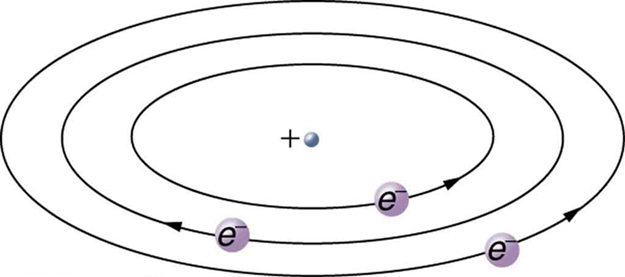
\includegraphics[scale=0.5]{rutherford-atom.jpeg}
\caption{Rutherford’s planetary model of the atom}
\end{figure}
\chapter{Radioisotopes}

\begin{itemize}
	\item A substance or object that emits nuclear radiation is said to be radioactive.
	\item Nuclear radiation is the emission of rays that originate in the nuclei of atoms and have other unique characterisitics.
	\item It consists of three types of radiation. Alpha, beta and gamma rays.
	\item All three types of nuclear radiation produce ionization in materials, but they penetrate different distances in materials—that is, they have different ranges.
	\item Radioisotopes are radio active isotopes of an element.
\end{itemize}
\begin{tcolorbox}[title=Ionizing radiation]
Ionizing radiation is defined as any form of radiation that produces ionization whether nuclear in origin or not, since the effects and detection of the radiation are related to ionization.
\end{tcolorbox}
\chapter{Biomedical application of radioisotopes}
\begin{itemize}
\item
A host of medical imaging techniques employ nuclear radiation.

\item Nuclear radiation can easily penetrate tissue; hence, it is a useful probe to monitor conditions inside the body.

\item Nuclear radiation depends on the nuclide and not on the chemical compound it is in, so that a radioactive nuclide can be put into a compound designed for specific purposes. The compound is said to be tagged. A tagged compound used for medical purposes is called a radiopharmaceutical.

\item Radiation detectors external to the body can determine the location and concentration of a radiopharmaceutical to yield medically useful information.

\item For example, certain drugs are concentrated in inflamed regions of the body, and this information can aid diagnosis and treatment.

\item Another application utilizes a radiopharmaceutical which the body sends to bone cells, particularly those that are most active, to detect cancerous tumors or healing points. Images can then be produced of such bone scans.

\item  Radioisotopes are also used to determine the functioning of body organs, such as blood flow, heart muscle activity, and iodine uptake in the thyroid gland.

\end{itemize}
\begin{figure}
\centering
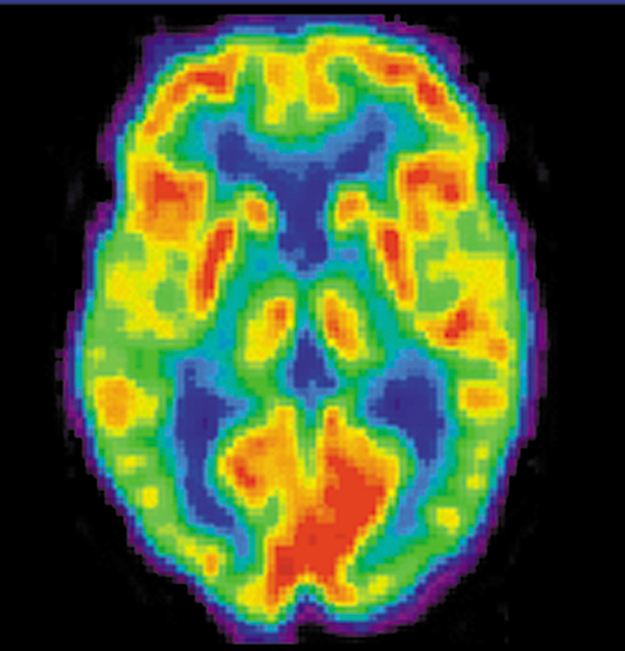
\includegraphics[scale=0.5]{radiomedicine.jpeg}
\caption{A radiopharmaceutical is used to produce this brain image of a patient with Alzheimer’s disease. Certain features are computer enhanced.}
\end{figure}

\section{Diagnosis}
\begin{itemize}
    \item  Many organs can be imaged with a variety of nuclear isotopes replacing a stable element by a radioactive isotope.
    \item One common diagnostic employs iodine to image the thyroid, since iodine is concentrated in that organ. The most active thyroid cells, including cancerous cells, concentrate the most iodine and, therefore, emit the most radiation. Conversely, hypothyroidism is indicated by lack of iodine uptake.
    \item Note that there is more than one isotope that can be used for several types of scans.
    \item Another common nuclear diagnostic is the thallium scan for the cardiovascular system, particularly used to evaluate blockages in the coronary arteries and examine heart activity. The salt TlCl can be used, because it acts like NaCl and follows the blood.
    \item Gallium-67 accumulates where there is rapid cell growth, such as in tumors and sites of infection. Hence, it is useful in cancer imaging. Usually, the patient receives the injection one day and has a whole body scan 3 or 4 days later because it can take several days for the gallium to build up.
\end{itemize}

\subsection{Single-photon-emission computed tomography(SPECT)}
\begin{itemize}
    \item Imaging techniques much like those in x-ray computed tomography (CT) scans use nuclear activity in patients to form three-dimensional images.

	Figure \ref{fig:spect} shows a patient in a circular array of detectors that may be stationary or rotated, with detector output used by a computer to construct a detailed image.

\item This technique is called single-photon-emission computed tomography(SPECT) or sometimes simply SPET.

\item The spatial resolution of this technique is poor, about 1 cm, but the contrast (i.e. the difference in visual properties that makes an object distinguishable from other objects and the background) is good.

\end{itemize}
\begin{figure}[htpb]
    \centering
    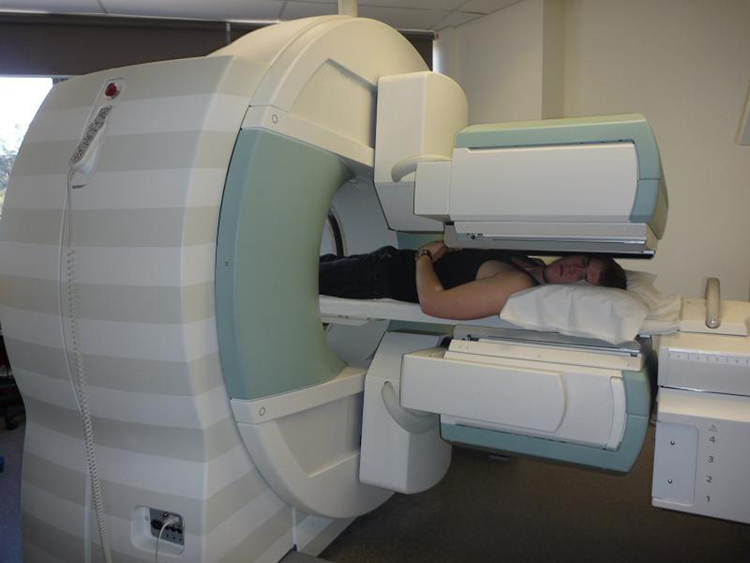
\includegraphics{spect.jpeg}
    \caption{SPECT uses a geometry similar to a CT scanner to form an image of the concentration of a radiopharmaceutical compound. (credit: Woldo, Wikimedia Commons)}%
    \label{fig:spect}
\end{figure}
\subsection{PET}
\begin{itemize}
	\item Images produced by $\beta + $ emitters have become important in recent years. When the emitted positron encounters an electron, mutual annihilation occurs, producing two gamma rays.
	    These gamma rays have identical  energies (0.511-MeV )
	    %the energy comes from the destruction of an electron or positron mass
	    and they move directly away from one another, allowing detectors to determine their point of origin accurately.
	\item The system is called positron emission tomography (PET). It requires detectors on opposite sides to simultaneously  detect photons and utilizes computer imaging techniques similar to those in SPECT and CT scans.

	\item  Examples of  $\beta + $ emitting isotopes used in PET are $^{11}C, ^{13}N, ^{15}O, $ \ and $ ^{18}F$ . This list includes C, N, and O, and so they have the advantage of being able to function as tags for natural body compounds.

	\item Its resolution of 0.5 cm is better than that of SPECT; the accuracy and sensitivity of PET scans make them useful for examining the brain’s anatomy and function.
	\item  The brain’s use of oxygen and water can be monitored with $^{15}O$. PET is used extensively for diagnosing brain disorders. It can note decreased metabolism in certain regions prior to a confirmation of Alzheimer’s disease. PET can locate regions in the brain that become active when a person carries out specific activities, such as speaking, closing their eyes, and so on.
\end{itemize}

\begin{figure}
\centering
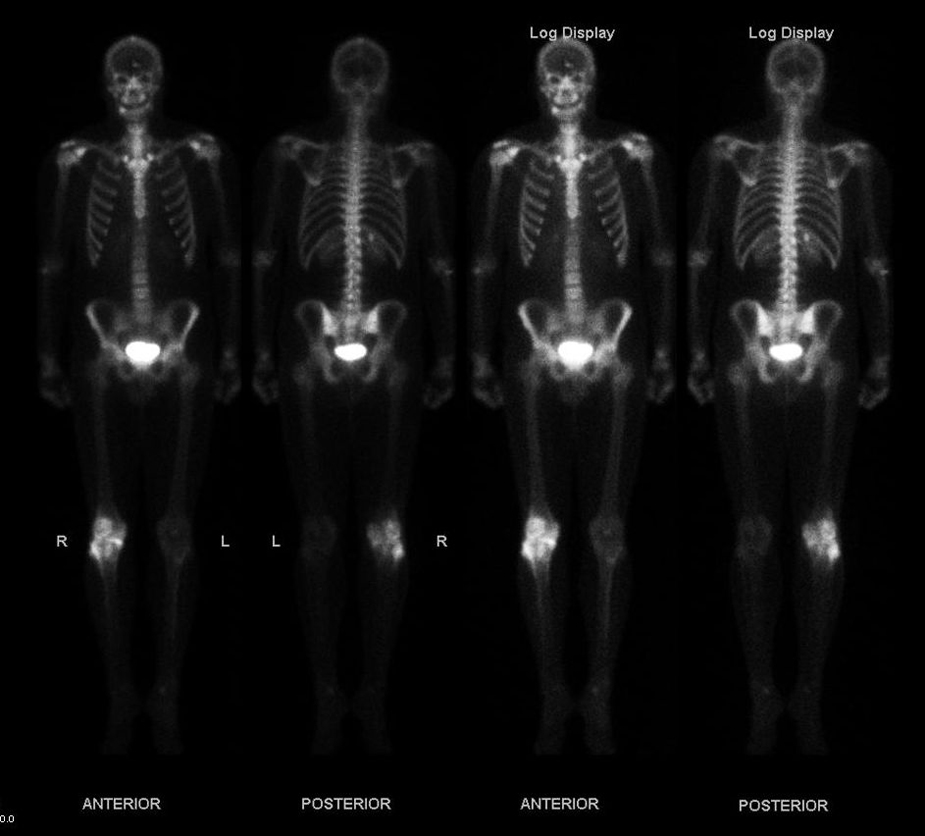
\includegraphics[scale=0.5]{gamma-scan.jpeg}
\caption{This image of the concentration of a radioactive tracer in a patient’s body reveals where the most active bone cells are, an indication of bone cancer. A short-lived radioactive substance that locates itself selectively is given to the patient, and the radiation is measured with an external detector. The emitted  gamma radiation has a sufficient range to leave the body—the range of alpha  and beta   is too small for them to be observed outside the patient.}
\end{figure}
\begin{figure}
\centering
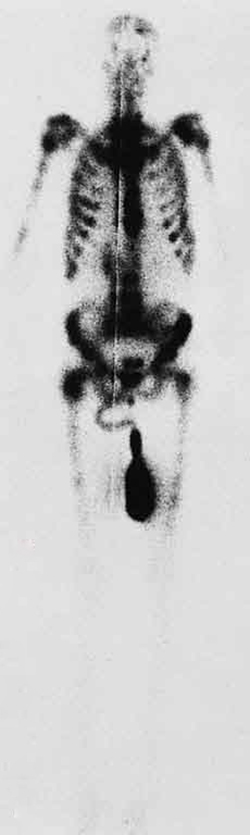
\includegraphics[scale=0.65]{gamma.jpeg}
\caption{ This is an image of the gamma rays emitted by nuclei in a compound that is concentrated in the bones and eliminated through the kidneys. Bone cancer is evidenced by nonuniform concentration in similar structures. For example, some ribs are darker than others.}
\end{figure}

\section{Use of radioisotopes in medicine}
Refer to text.

%\begin{itemize}
	%\item If radio sodium ($^{24}{Na}$) is injected at one end of the body, it
%can be detected with in a few second at the other part. The
%flow of blood can thus be followed and any constrictions in
%blood vessels are readily detected.

%\item  Radio iodine ($^{131}I$) is useful in medicine because it is thought
%to accumulate in thyroid gland. Being an emitter radioactive
%iodine is useful in locating deep seated brain tumor and
%malignant thyroid tumors. Ordinarily thyroid iodine deficiency
%can also be treated in a controlled manner using (131I) as the
%tracer nuclide. The isotope is helpful to the diagnosing and
%determining whether the uptake of iodine by the gland is
%normal. If the thyroid gland is not functioning the uptake will
%be less than normal. If the gland is hyperfunctional the uptake
%of iodine will be greater than normal.

%\item It has been similarly useful in localizing brain tumors. For
%this human serum albumin is tagged with 131I and injected new
%tumor growth has an affinity for the serum albumin and it
%collects in these tissues. The tumor is then located by employing
%a sterile counting probe.


%\item The tumor in breast is similarly detected by using radio-
%phosphorus (32 P). It has also been reported as useful
%therapeutically is polycythemia vera and leukemia.


%\item Radioactive cobalt ( 60 Co) emits radiations similar to that
%obtained by X-ray. Because cobalt is a metal it can be shaped
%into various forms and is particularly used in treating tumors
%locally. Cobalt wires have been introduced directly into the
%tissues. One report indicates successful results from the use
%of radioactive wires placed in internal mammary artery of
%patient with breast tumor after the primary tumor has been
%removed. 60 Co is also used to irradiate tissues from the distance.
%The is called teletherapy.

%\item Radio-iron can be given experimentally to determine the tissues
%in which iron is stored and utilized. Since some of the radio-
%iron is incorporate in the hemoglobin, tracer studies related
%to erythrocyte life cycle have been reported.

%\end{itemize}


\chapter{Detecting Radiation}
\begin{itemize}
	\item
Ionizing radiation, such as X-rays, alpha rays, beta rays, and gamma
rays, remains undetectable by the senses, and the damage it causes
to the body is cumulative, related to the total dose received.
\item Therefore,
workers who are exposed to radiation, such as radiographers, nuclear
power plant workers, doctors using radiotherapy, workers in
laboratories using radionuclides are
required to wear instrument which can keep a record of their exposure,
to verify that it is below legally prescribed limits.
 \item Ionizing radiations
can be measures or monitored by dosimeters, Geiger counters and
scintillation counters.
\end{itemize}

%\section{Photographic films}
%Photographic film is still the most common detector of ionizing radiation, being used routinely in medical and dental x rays as shown in \ref{fig:filmbadge} .  The mechanism for film exposure by ionizing radiation is similar to that by photons.

%\begin{figure}
    %\centering
    %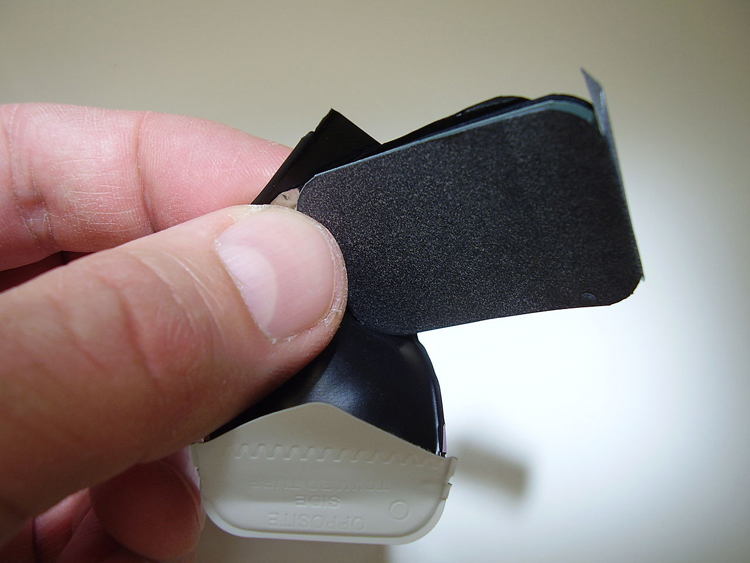
\includegraphics[scale=0.5]{filmbadge.jpeg}
    %\caption{Film badges contain film similar to that used in this dental x-ray film and is sandwiched between various absorbers to determine the penetrating ability of the radiation as well as the amount.}%
    %\label{fig:filmbadge}
%\end{figure}
%\section{Geiger-Muller counter}
%\begin{itemize}
    %\item  Another very common radiation detector is the Geiger tube. The clicking and buzzing sound heard usually is an audio output of events detected by a Geiger counter shown schematically in \ref{gm}.

    %\item A conducting cylinder with a wire along its axis is filled with an insulating gas so that a voltage applied between the cylinder and wire produces almost no current.
    %\item Ionizing radiation passing through the tube produces free ion pairs (each pair consisting of one positively charged particle and one negatively charged particle) that are attracted to the wire and cylinder, forming a current that is detected as a count.

    %\item The word count implies that there is no information on energy, charge, or type of radiation with a simple Geiger counter. They do not detect every particle, since some radiation can pass through without producing enough ionization to be detected. However, Geiger counters are very useful in producing a prompt output that reveals the existence and relative intensity of ionizing radiation.


%\end{itemize}
%\begin{figure}
%\centering
%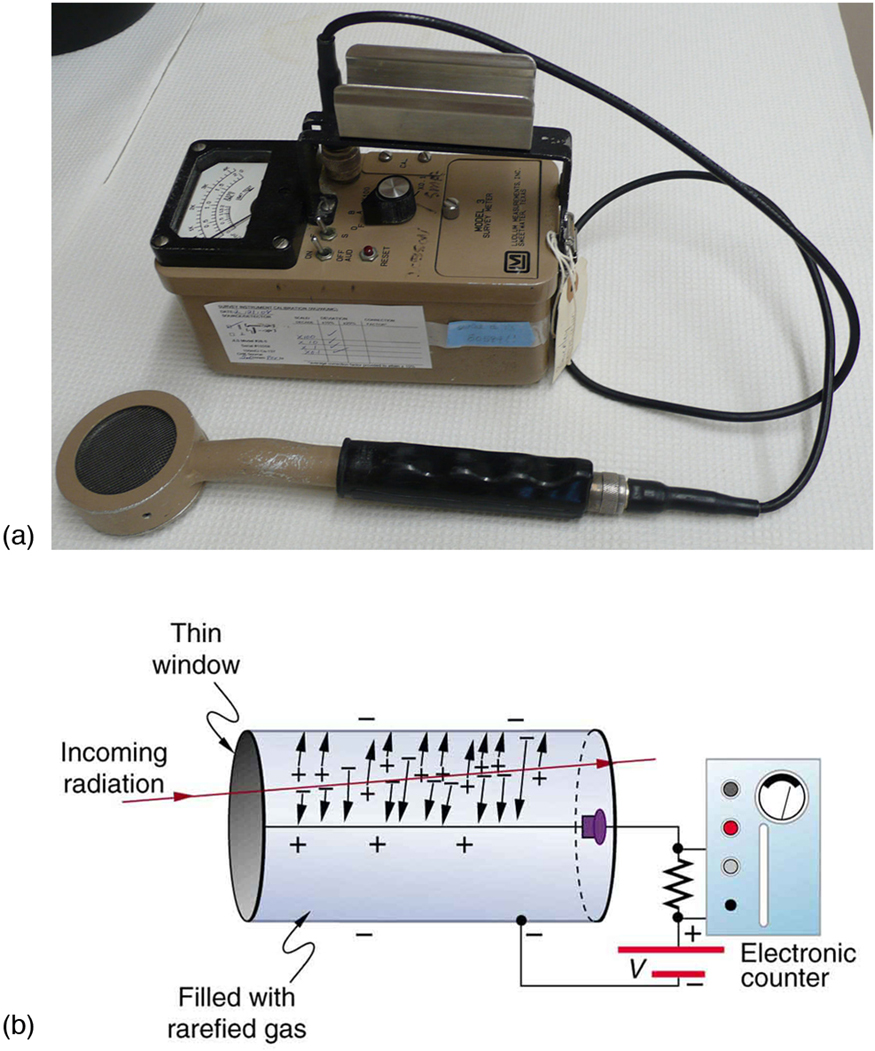
\includegraphics[scale=0.45]{gm.jpeg}
%\caption{(a) Geiger counters such as this one are used for prompt monitoring of radiation levels, generally giving only relative intensity and not identifying the type or energy of the radiation. (b) Voltage applied between the cylinder and wire in a Geiger tube causes ions and electrons produced by radiation passing through the gas-filled cylinder to move towards them. The resulting current is detected and registered as a count.}
%\label{gm}
%\end{figure}
%\section{Scintillation counters}
%\begin{itemize}
    %%\item Another radiation detection method records light produced when radiation interacts with materials.
%%The energy of the radiation is sufficient to excite atoms in a material that may fluoresce, such as the phosphor .

    %\item Scintillators use a complex collaborative process to convert radiation energy into light.
    %\item Scintillators may be liquid or solid, and they can be very efficient. Their light output can provide information about the energy, charge, and type of radiation.
    %\item Scintillator light flashes are very brief in duration, enabling the detection of a huge number of particles in short periods of time. Scintillator detectors are used in a variety of research and diagnostic applications.
    %\item Light from a scintillator is converted into electrical signals by devices such as the photomultiplier tube shown schematically in \ref{scintillator}.
    %\item Light entering the photomultiplier strikes a metal plate, ejecting an electron that is attracted by a positive potential difference to the next plate, giving it enough energy to eject two or more electrons, and so on. The final output current can be made proportional to the energy of the light entering the tube, which is in turn proportional to the energy deposited in the scintillator. Very sophisticated information can be obtained with scintillators, including energy, charge, particle identification, direction of motion, and so on.

%\end{itemize}
%\begin{figure}
    %\centering
    %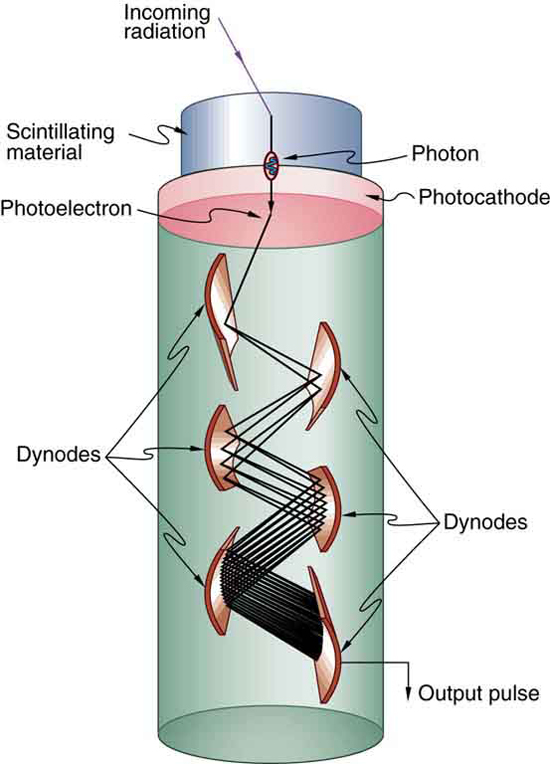
\includegraphics[scale=0.5]{scintillator.jpeg}
    %\caption{Scintillator}%
    %\label{scintillator}
%\end{figure}
%\subsection{Dosimeter}
 %Dosimeters measure an absolute dose received over
%a period of time.
 %Common types of wearable dosimeters
%for ionizing radiation include:
%\begin{itemize}
%\item Ion chamber dosimeter
%\item  Film badge dosimeter
%\item  Thermoluminescent dosimeter
%\item Solid state dosimeter
%%\item Solid state (MOSFET or silicon diode) dosimeter
%\end{itemize}\
%\begin{figure}
%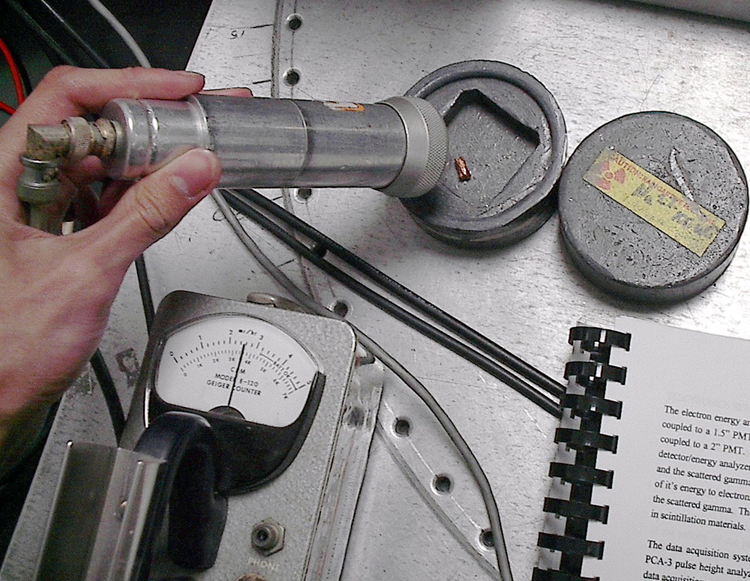
\includegraphics[scale=0.5]{dosimeter.jpeg}
%\centering
%\caption{Dosimeters are personal radiation monitors that detect the amount of radiation by the discharge of a rechargeable internal capacitor. The amount of discharge is related to the amount of ionizing radiation encountered.}
%\end{figure}
%Ion-chamber dosimeters resemble pens, and can
%be clipped to one’s clothing.
%Ion-
%chamber dosimeters must be periodically recharged, and the result
%logged.

%Film-badge dosimeters enclose a piece of photographic film,
%which will become exposed as radiation passes through it.
%Film-badge dosimeters must be developed as photographic emulsion so the exposures can be counted and logged; once developed, they are discarded.


%Another type of dosimeter is the TLD (Thermoluminescent dosimeter). These dosimeters contain crystals that emit visible light when heated, in direct proportion
%to their total radiation exposure.

%Common types of wearable dosimeters for ionizing radiation include:

%\subsection{Gieger counters}
%%\begin{itemize}
	%%\item
	 %Geiger counters are used to detect ionizing
%radiation (usually beta particles and gamma rays, but certain
%models can detect alpha particles). An inert gas-filled tube (usually
%helium, neon or argon with halogens added) briefly conducts
%electricity when a particle or photon of radiation makes the gas
%conductive. The tube amplifies this conduction by a cascade effect
%and outputs a current pulse, which is then often displayed by a
%needle or lamp and/or audible clicks. Modern instruments can
%report radioactivity over several orders of magnitude.
%\end{itemize}

%\subsection{Scintillation counter}
%A scintillation counter measures ionizing
%radiation. The sensor, called a scintillator, consists of a transparent
%crystal, usually phosphor, plastic (usually containing anthracene),
%or organic liquid (see liquid scintillation counting) that fluoresces
%when struck by ionizing radiation. A sensitive photomultiplier tube
%(PMT) measures the light from the crystal. The PMT is attached
%to an electronic amplifier and other electronic equipment to count
%and possibly quantify the amplitude of the signals produced by
%the photomultiplier.



\chapter{Radiation Hazards}
\begin{itemize}
    \item All the effects of ionizing radiation on biological tissue can be understood by knowing that ionizing radiation affects molecules within cells, particularly DNA molecules.

    \item DNA contains codes that check whether the DNA is damaged or can repair itself. It is like an auto check and repair mechanism. This repair ability of DNA is vital for maintaining the integrity of the genetic code and for the normal functioning of the entire organism.
    \item Ionizing radiation can induce damage to the ability of cells to repair DNA. As a result of this,

	\begin{itemize}
\item The cell can go into an irreversible state of dormancy, known as senescence.
\item The cell can commit suicide, known as programmed cell death.
\item The cell can go into unregulated cell division leading to tumors and cancers.

\end{itemize}

\item Since ionizing radiation damages the DNA, which is critical in cell reproduction, it has its greatest effect on cells that rapidly reproduce, including most types of cancer. Thus, cancer cells are more sensitive to radiation than normal cells and can be killed by it easily.
\item Cancer is characterized by a malfunction of cell reproduction, and can also be caused by ionizing radiation. Without contradiction, ionizing radiation can be both a cure and a cause.

\item The large-scale effects of radiation on humans can be divided into two categories: immediate effects and long-term effects.
    \begin{itemize}
 \item
Immediate effects are explained by the effects of radiation on cells and the sensitivity of rapidly reproducing cells to radiation.
\item The first clue that a person has been exposed to radiation is a change in blood count, which is not surprising since blood cells are the most rapidly reproducing cells in the body.
\item At higher doses, nausea and hair loss are observed, which may be due to interference with cell reproduction. Cells in the lining of the digestive system also rapidly reproduce, and their destruction causes nausea.
When the growth of hair cells slows, the hair follicles become thin and break off.

\item
The two known long-term effects of radiation are cancer and genetic defects. Both are directly attributable to the interference of radiation with cell reproduction.
    \end{itemize}

\item  High doses cause significant cell death in all systems, but the lowest doses that cause fatalities do so by weakening the immune system through the loss of white blood cells.
\end{itemize}

\chapter{Radiation Units}

\begin{itemize}
    \item  All effects of radiation are assumed to be directly proportional to the amount of ionization produced in the biological organism.
    \item The amount of ionization is in turn proportional to the amount of deposited energy. Therefore, we define a radiation dose unit called the rad, as 1/100 of a joule of ionizing energy deposited per kilogram of tissue,

$1 \ rad = 0.01 J/kg$.

\item While calculating radiation doses, you divide the energy absorbed by the mass of affected tissue. You must specify the affected region, such as the whole body or forearm in addition to giving the numerical dose in rads. The SI unit for radiation dose is the gray (Gy), which is defined to be

$1 \ Gy =1 J/kg = 100 \ rad$.

\item The effects of ionizing radiation may be directly proportional to the dose in rads, but they also depend on the type of radiation and the type of tissue. That is, for a given dose in rads, the effects depend on whether the radiation is $\alpha, \beta, \gamma $, x-ray, or some other type of ionizing radiation.

\item If the range of the radiation is small, as it is for alpha rays, then the ionization and the damage created is more concentrated and harder for the organism to repair, so short-range particles have greater biological effects.
\item
The relative biological effectiveness (RBE) or quality factor (QF) is different for different types of ionizing radiation—the effect of the radiation is directly proportional to the RBE.

\item A dose unit more closely related to effects in biological tissue is called the roentgen equivalent man or rem and is defined to be the dose in rads multiplied by the relative biological effectiveness.

$ rem = rad \times RBE$

The SI equivalent of the rem is the sievert (Sv), defined to be

$ Sv = \ Gy \times  RBE$



\end{itemize}

\chapter{Radiation protection}
\begin{itemize}
    \item  Laws regulate radiation doses to which people can be exposed.
    \item The greatest occupational whole-body dose that is allowed depends upon the country and is about 20 to 50 mSv/y and is rarely reached by medical and nuclear power workers.
    \item Higher doses are allowed for the hands. Much lower doses are permitted for the reproductive organs and the fetuses of pregnant women.
    \item Inadvertent doses to the public are limited to 1/10 of occupational doses, except for those caused by nuclear power, which cannot legally expose the public to more than 1/1000 of the occupational limit or 0.05 mSv/y (5 mrem/y).
    \item Extensive monitoring with a variety of radiation detectors is performed to assure radiation safety. Increased ventilation in uranium mines has lowered the dose there to about 1 mSv/y.

    \item To physically limit radiation doses, we use shielding, increase the distance from a source, and limit the time of exposure.
	\begin{itemize}
    \item  Shielding absorbs radiation and can be provided by any material, including sufficient air.
    \item The greater the distance from the source, the more the radiation spreads out.
    \item The less time a person is exposed to a given source, the smaller is the dose received by the person.

\end{itemize}
    \item Doses from most medical diagnostics have decreased in recent years due to faster films that require less exposure time.
\end{itemize}
\end{document}
